\chapter{Аналитический раздел}
\label{cha:analysis}
%
% % В начале раздела  можно напомнить его цель
%
Алгоритмы, с которыми приходится иметь дело при параллельном программировании гораздо сложнее, чем аналогичные последовательные алгоритмы. Часть проблем касается распараллеливания самого алгоритма (например, как разбить процесс на задачи и как поставить им в соответствие физические процессоры), часть касается оптимального использования вычислительных ресурсов (баланс загрузки процессоров, межпроцессные взаимодействия, доступ к кэшу). Для разработки высокопроизводительных приложений программисту не только очень хорошо знать структуру самого приложения, но и структуру аппаратной платформы, а зачастую и программной (особенности операционной системы, компилятора и.т.д.).
Итак, уровень знаний, необходимый для разработки высокопроизводительных параллельных программ выше, чем для последовательных программ. Параллельное программирование может быть очень мучительным и запутанным. В добавок отладка параллельной программы и поиск критических мест также трудоёмкий и длительный процесс.
Из-за этих причин программирование для массивно параллельных машин считается непростым делом, и в значительной степени причиной этому служит недостаток инструментария по сравнению с последовательными машинами. Для того, чтобы понять поведение и внутреннюю логику параллельных программ и помочь программисту выявить потенциальные слабые места (например, ограничения по межпроцессным взаимодействиям) необходимы средства контроля хода выполнения параллельной программы. Они могут использоваться для сравнения производительности схожих программ или помогать при отладке.


% Обратите внимание, что включается не ../dia/..., а inc/dia/...
% В Makefile есть соответствующее правило для inc/dia/*.pdf, которое
% берет исходные файлы из ../dia в этом случае.



\section{Парадигмы параллельного программирования}
\subsection{Структура и характеристики параллельных алгоритмов}
Любой параллельный алгоритм (программа) состоит из блоков последовательных и параллельных вычислений. Последовательная часть программы (называется критическим сечением) – это последовательность операторов, которая должна выполняться только одним процессором. За критическим сечением обычно следует ветвление, инициирующее параллельно выполняемые участки программы (параллельные сегменты). В месте соединения параллельных сегментов выполняется синхронизация и параллельные сегменты возвращаются к критическому сечению. Синхронизация требуется для того, чтобы вычисления в параллельных сегментах закончились прежде, чем начнется выполнение последовательной части. 

\subsection{Программные парадигмы}

При параллельном программировании появляются дополнительные сложности (по сравнению с последовательным программированием): возникает необходимость управлять несколькими процессорами и координировать межпроцессорные вызовы. В общем случае параллельная программа представляет собой ряд заданий, работающих параллельно друг другу и взаимодействующих между собой. Существует несколько парадигм (моделей) программирования при создании параллельных алгоритмов. Наиболее распространенными парадигмами являются модель передачи сообщений и модель разделяемой памяти.


\subsection{Проектирование параллельных алгоритмов}
Несмотря на то, что проектирование параллельных алгоритмов есть процесс творческий и в общем случае достаточно сложно рекомендовать универсальный рецепт, следует все же привести общую методологию проектирования параллельных алгоритмов, которая в значительной степени оградит проектировщика от потенциальных ошибок.

\begin{figure}[h!]
	\centering
	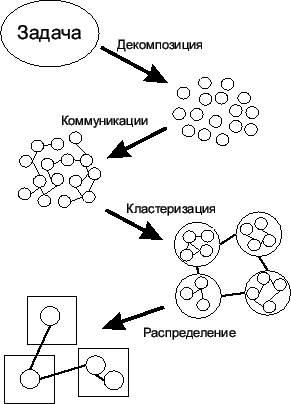
\includegraphics[width=0.4\textwidth]{img/img1.png}
	\caption{Методология проектирования параллельных алгоритмов}
	\label{fig:spire05}
\end{figure}

Описываемая методология проектирования предлагает подход к распараллеливанию, который рассматривает машинно-независимые аспекты реализации алгоритма, такие как параллелизм, на первой стадии, а особенности проектирования, связанные с конкретным параллельным компьютером, - на второй. Данный подход разделяет процесс проектирования на четыре отдельных этапа: декомпозиция (partitioning), коммуникации (communications), кластеризация (agglomeration) и распределение (mapping). Первые два этапа призваны выделить в исходной задаче параллелизм и масштабируемость, остальные этапы связаны с различными аспектами производительности алгоритма. Рисунок 1.1 иллюстрирует процесс проектирования параллельного алгоритма.  
Сформулируем кратко содержание этих этапов. 
\subsubsection{Декомпозиция} 
Общая задача вычислений и обработки данных делится на меньшего размера подзадачи. При этом игнорируются проблемы практической реализации, например, число процессоров используемого в будущем компьютера. Напротив, все внимание сосредотачивается на возможном параллелизме исходной задачи. 
\subsubsection{Коммуникации}
Определяется требуемая связь между подзадачами, ее структура и конкретные алгоритмы коммуникаций. 
\subsubsection{Кластеризация} 
Структура подзадач и коммуникаций оценивается с учетом требований производительности алгоритма и затрат на реализацию. Если необходимо, отдельные подзадачи комбинируются в более крупные с целью улучшения производительности и снижения затрат на разработку. 
\subsubsection{Распределение} 
Каждая подзадача назначается определенному процессору, при этом стараются максимально равномерно загрузить процессоры и минимизировать коммуникации. Распределение может быть статическим или формироваться в процессе выполнения программы на основе алгоритмов балансировки загрузки (load balancing algorithms). 
Следует заметить, что при прохождении последних двух этапов необходимо учитывать архитектуру параллельного компьютера, имеющегося в распоряжении разработчика, другими словами параллельный алгоритм должен быть адекватен используемой параллельной системе. 
\section{Дизеринг при помощи диффузии ошибок}
Метод, обладающий наилучшим качеством среди представленных, - метод рассеивания ошибок. Но так же он, к сожалению, самый медленный.\cite{Dh} Существуют несколько вариантов этого алгоритма, причем скорость алгоритма обратно пропорционально качеству изображения.\cite{Dh}
Суть алгоритма: для каждой точки изображения находим ближайший возможный цвет. Затем мы рассчитываем разницу между текущим значеним и ближайшим возможным. Эта разница и будем нашем значением ошибки.Это значение ошибки мы распределяем между соседними элементами, которые мы ещё не посещали. Для последних точек ошибка распределяется между уже посещенными точками.
\subsection{Характеристики производительности параллельного алгоритма}
Задачей программиста является проектирование и реализация программ, которые удовлетворяют требованиям пользователя в смысле производительности и корректной работы. Производительность является достаточно сложным и многосторонним понятием. Кроме времени выполнения программы и масштабируемости следует также анализировать механизмы, отвечающие за генерацию, хранение и передачу данных по сети, оценивать затраты, связанные с проектированием, реализацией, эксплуатацией и сопровождением программного обеспечения. Существуют весьма разнообразные параметры, влияющие на производительность вычислительной системы. Среди них наиболее значимыми являются: требования по памяти, производительность сети, время задержки при передаче данных (latency time), переносимость, масштабируемость, затраты на проектирование, реализацию, отладку, требование к аппаратному обеспечению и т.д. Критериями, по которым оценивается производительность, являются время выполнения программы, ускорение и эффективность.
Относительная важность различных параметров будет меняться в зависимости от природы вычислительной системы и поставленной задачи. Специфика конкретной задачи может требовать высоких показателей для каких-либо определенных критериев, в то время как остальные должны быть оптимизированы или полностью игнорированы. 
Ниже мы рассмотрим лишь две характеристики производительности, а именно, эффективность и ускорение, поскольку они наиболее часто используются при анализе производительности параллельных алгоритмов.
\begin{equation}
S_{p0} = \frac{T_{0}}{T_{p}}

\label{F:F1}
\end{equation}
\subsection{Фильтр Флойда-Cтейнберга }
Каждый пиксель распределяет свою ошибку на соседние с ним пиксели. Коэффициенты были подобраны таким образом, что в районах с  интенсивностью 1/2 от общего количество оттенков, изображение выглядело похожим на шахматную доску.\\
$  \begin{vmatrix}
\boxminus & \boxtimes & 7\\
3 & 5 & 1
\end{vmatrix}$ (1/16)
\subsection{"Ложный"  фильтр Флойда-Стейнберга }
В случае сканирования слева-направо этот фильтр порождает большое количество артефактов.Чтобы получить изображение с меньшим количеством артефактов, нужно чётные строки сканировать справа-налево, а нечетные строки сканировать слева-направо.\\
$\begin{vmatrix}
\boxtimes & 3 \\
3 & 2 
\end{vmatrix} $(1/8)

\subsection{Фильтр Джарвиса,Джунка и Нинка}
В случае когда фильтры Флойда-Стейдберга дают недостаточно хороший результат, применяются фильтры с более широким распределением ошибки. Фильтр Джарвиса, Джунка и Нинка требует связи с 12 соседями, что очевидно ведет в большим затратам памяти и времени\cite{Dh}:\\
$\begin{vmatrix}
\boxminus & \boxminus & \boxtimes & 7 & 5\\
3 & 5 & 7 & 5 &3 \\
1 & 3 & 5 & 3 & 1 
\end{vmatrix}$(1/48)

\subsection{Фильтр Стаки}
Фильтр разработан на основе фильтра Джарвиса, Джунка и Нинка.После такого как мы вычислим 8/42 ошибки, остальные значения можно получить при помощи побитовых сдвигов, тем самым сокращая время работы алгоритма.\\
$\begin{vmatrix}
\boxminus & \boxminus & \boxtimes & 8 & 4 \\
2 & 4 & 8 & 4 & 2 \\
1 & 2 & 4 & 2 & 1

\end{vmatrix}$ (1/42)

\subsection{Фильтр Бурка}
Стаки. Результат можно получить чуть быстрее за счет использования побитовых операций.\\
$\begin{vmatrix}
\boxminus &  \boxminus & \boxtimes  & 8 & 4\\
2 & 4 & 8 & 4 & 2
\end{vmatrix}$ (1/32)\\
Существует много различных вариантов фильтро дизеринга при помощи диффузии ошибок, здесь приведены наиболее  популярные алгоритмы.\cite{Dh}
\section{Прочие виды дизеринга}
Компьютерная графика не стоит на месте и завидной переодичностью появляются всё новые виды дизеринга, не укладывающиеся в привычную классификацию.
\subsection{Алгоритм Юлиомы}
Существует три вариации этого алгоритма \cite{Wiki_Yliluoma} значительно отличающиеся друг от друга. Основная идея этих алгоритмов заключается в оптимальном подборе цвета ограниченной цветовой палитры, основываваясь на визуальном восприятии этого цвета, а не на его числовом коде. Отличается от остальных алгоритмов значительными временными затратами, что делает применение этого алгоритма для решения практических задач затруднительным.

\section{Выбор оптимального класса алгоритма}
Вышеприведенные методы упорядочены по качеству получаемого на выходе изображения, однако, такие соображения как время, экономия памяти и прочие являются определяющими при выборе алгоритма\cite{Dh}.
На основе вышеприведенных данных сравним классы алгоритмов дизеринга.
\begin{tabular}{|@{\hspace*{2mm}}l||*{3}{c|}}\hline
	\multicolumn{1}{|@{}l||}{\backslashbox[0pt][l]{Вид алгоритма}{Характеристика }}
	&\makebox[4em]{Cкорость}&\makebox[4em]{Качество}&\makebox[5em]{Доп память}
	%	&\makebox[3em]{6/3}&\makebox[3em]{6/4}
	\\\hline\hline
	Cлучайный&+&-&-\\\hline
	Шаблонный &+-&-+&+\\\hline
	Упорядоченный&-+&+-&-\\\hline
	Диффузия ошибок&-&+&+\\\hline
	Остальные &-&+&+\\\hline
\end{tabular}
\bigskip
\\
Самым быстрым классом алгоритмов дизеринга является случайный дизеринг.Однако, качество получаемых при помощи изображений низко. Алгоритмы упорядоченного дизеринга позволяют получить изображения более высокого качества, однако работают более медленно и требуют дополнительных затрат. В зависимости от вычислительных ресурсов и требуемого результата рациональным будет применение различых алгоритмов.
\section{Оценка алгоритмов}
n - количество пикселей в изображении

\begin{tabular}{|@{\hspace*{2mm}}l||*{3}{c|}}\hline
	\multicolumn{1}{|@{}l||}{\backslashbox[0pt][l]{Вид алгоритма}{Характеристика }}
	&\makebox[4em]{Время}&\makebox[4em]{Память}
	%	&\makebox[3em]{6/3}&\makebox[3em]{6/4}
	\\\hline\hline
	Cлучайный&O(n)&O(1)\\\hline
	Упорядоченный&O(n)&O(1)\\\hline
	Диффузия ошибок&O(n)&O(n)\\\hline
	Первый алгоритм Юлиомы &O($n^3$)&O(n)\\\hline
\end{tabular}


%%% Local Variables:
%%% mode: latex
%%% TeX-master: "rpz"
%%% End:
